\section{Rede Neural}\label{cap:abordagem_rede_neural}

Essa abordagem consiste em usar uma Rede Neural que tem como entrada o estado do
jogo (todas as posições, orientações, velocidades e o comando do juiz) e como
saída o estado do time adversário (todas as posições, orientações e velocidades
dos robôs do time adversário), que visa prever as ações imediatas do adversário.
Essa rede deve ser treinada para prever um time específico usando os
\textit{logs} das partidas do torneio de 2013 da \textit{RoboCup}.

\subsection{Teste de conceito}

% TODO[jansegre] observação em <posição da bola>

Para teste de conceito o problema foi reduzido a prever a posição da bola. Foi
implementado uma Rede Neural \textit{feedforward} com uma camada oculta cujo
número de nós foi variado entre 8 e 320. Os nós de entrada foram 4: posições $x$
e $y$, e velocidades em $x$ e $y$, como os \textit{logs} não possuem informação
de velocidade essa foi calculada usando a diferença entre dois quadros
consecutivos. São 2 nós de saída: as posições $x$ e $y$, do próximo quadro. Foi
usada ativação sigmoid simétrica. Nessa implementação o treinamento convergiu
para um erro muito alto, como pode ser visto abaixo na saída (resumida) do
treinamento com 32 nós ocultos, é usado o erro médio quadrático e a unidade de
distância é o milímetro.

% saída do treinamento
\lstinputlisting{../train.log}

Esse problema não era esperado, foi decidido que seria necessário analisar
melhor os dados de treinamento para entender os motivos do ocorrido. Para tanto
foi modificada uma ferramenta desenvolvida no laboratório, originalmente usada
para visualizar as partidas em tempo real, a fim de visualizar os \textit{logs}
das partidas. Ao inspecionar esses logs notou-se dois tipos de irregularidades
relevantes para o treinamento, mostradas na figura~\ref{fig:logs}.

%\begin{figure}[thpb]
%  \centering
%  \begin{subfigure}[b]{0.49\textwidth}
%    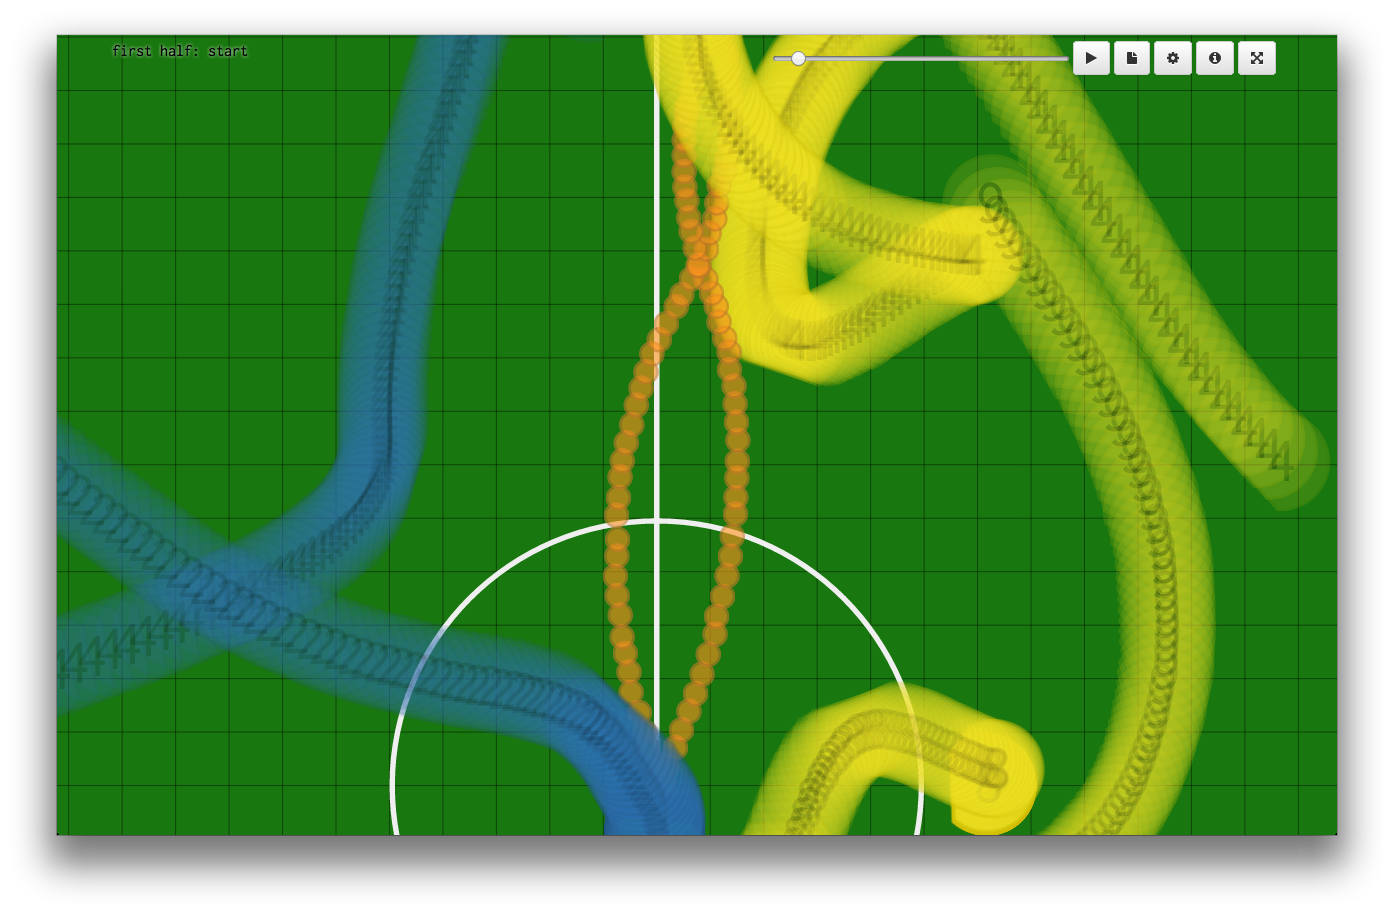
\includegraphics[width=\textwidth]{figuras/log_rastro.png}
%    \caption{Rastro duplo divergente}\label{fig:log_rastro}
%  \end{subfigure}
%  \begin{subfigure}[b]{0.49\textwidth}
%    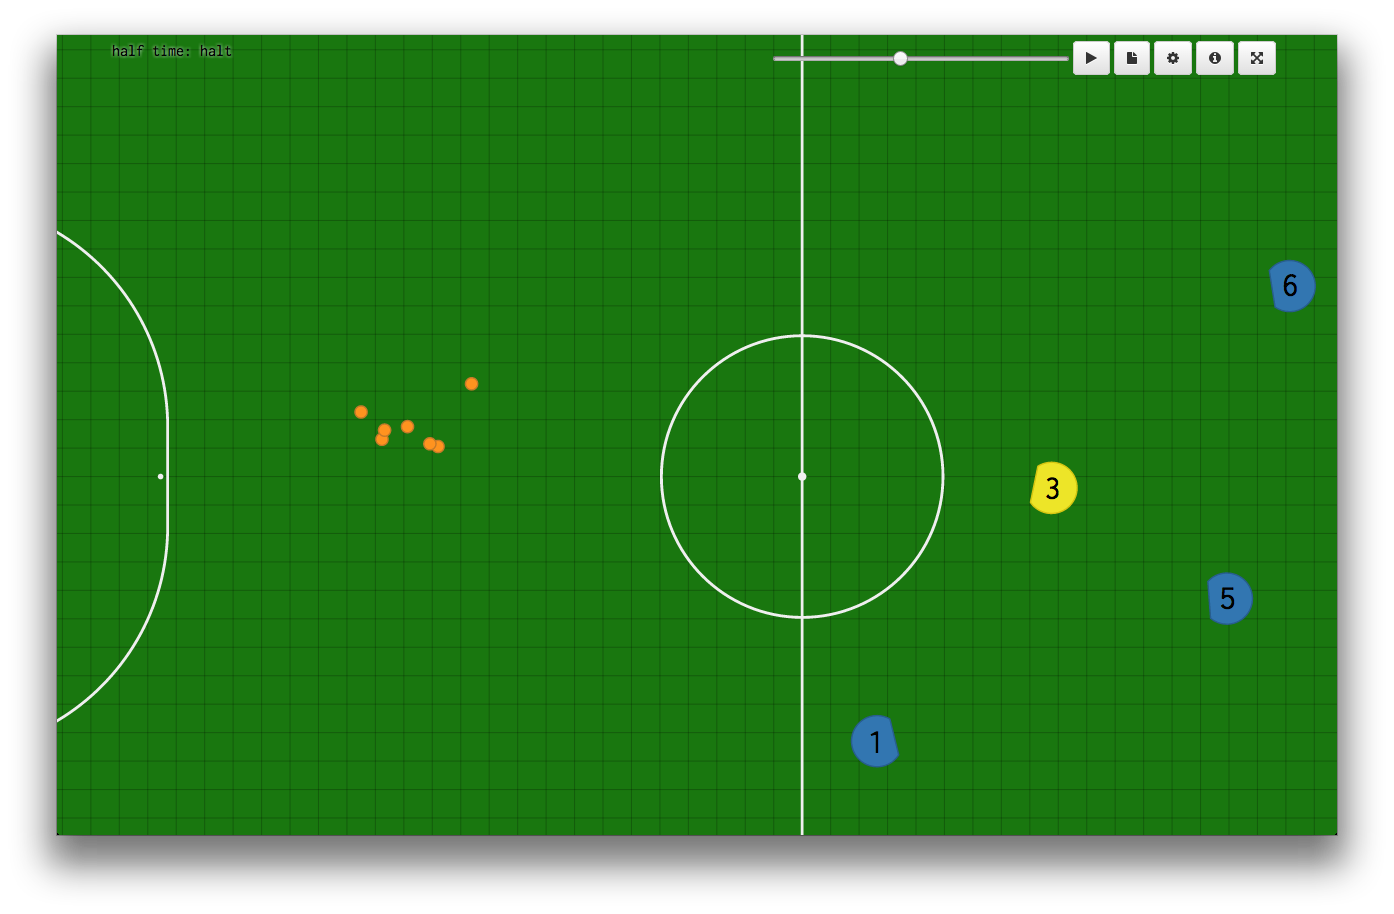
\includegraphics[width=\textwidth]{figuras/log_multi.png}
%    \caption{Objetos "fantasmas"}\label{fig:log_multi}
%  \end{subfigure}
%  \caption{Análise dos logs.}\label{fig:logs}
%\end{figure}

A figura~\ref{fig:log_rastro} mostra o problema que ocorre numa faixa no meio do
campo: a posição dos objetos (robôs e bola) oscila quadro a quadro. O motivo
desse problema é o fato das duas câmeras que capturam os dados possuírem uma
área de interseção e devido a diferenças sutis na calibração a posição dos
objetos difere quando vista de câmeras distintas. Uma saída trivial seria
ignorar os dados de uma das câmeras, mas isso é não é desejado pois uma parte
fundamental do estado do jogo estaria sendo ignorada.

Já na figura~\ref{fig:log_multi}, pode ser observado o segundo problema: há
momentos em que vários objetos "fantasmas" aparecem, isto é, são detectados
objetos que não existem no campo físico. O efeito disso é que a posição da bola
muda drasticamente para pontos que não fazem sentido.

A abordagem da rede neural, apesar de ocultar a semântica da relação dos fatores
analisados, parece bem apta a resolver o problema. Porém é necessário contornar
o problema dos dados de treinamento para poder implementar uma solução de fato.

% vim: tw=80 et ts=2 sw=2 sts=2
